\section{Exploratory data analysis}

\subsection{Data description}

The dataset used in this study was extracted from the project MonitorAr
\cite{dataset-rio-ar-quality}. The table contains hourly data observations, separated by
pollutant, weather condition, and monitoring stations' characteristics from
the city of Rio de Janeiro. Table
\ref{tab:measured-data} informs the most important variables used, and Table
\ref{tab:pollutants-measured} indicates the measured pollutants. The events were collected between January 1,
2011,
and March 31, 2021. A total of 661,662 records were used. 

\begin{table*}[t]
    \centering
    \begin{tabular}{c|c|c|c|}
        \cline{2-4}
                                                                                 & \textbf{Name} & \textbf{Type} & \textbf{Description}              \\ \hline
        \multicolumn{1}{|c|}{\multirow{7}{*}{\textbf{Meterological conditions}}} & Chuva         & float         & Rainfall (mm)                     \\ \cline{2-4} 
        \multicolumn{1}{|c|}{}                                                   & Pres          & float         & Atmospheric Pressure (mbar)       \\ \cline{2-4} 
        \multicolumn{1}{|c|}{}                                                   & RS            & float         & Solar radiation (w/m2)            \\ \cline{2-4} 
        \multicolumn{1}{|c|}{}                                                   & Temp          & float         & Temperature (°C)                  \\ \cline{2-4} 
        \multicolumn{1}{|c|}{}                                                   & UR            & float         & Relative humidity (\%)            \\ \cline{2-4} 
        \multicolumn{1}{|c|}{}                                                   & Dir\_Vento    & float         & Wind direction (°)                \\ \cline{2-4} 
        \multicolumn{1}{|c|}{}                                                   & Vel\_Vento    & float         & Wind speed (m/s)                  \\ \hline
        \multicolumn{1}{|c|}{\multirow{5}{*}{\textbf{Measurement conditions}}}   & Data          & datetime      & Measurement date and hour         \\ \cline{2-4} 
        \multicolumn{1}{|c|}{}                                                   & CodNum        & ineger        & Number of the monitoring station  \\ \cline{2-4} 
        \multicolumn{1}{|c|}{}                                                   & Estação       & string        & Name of the monitoring station    \\ \cline{2-4} 
        \multicolumn{1}{|c|}{}                                                   & Lat           & float         & Latitude position of the station  \\ \cline{2-4} 
        \multicolumn{1}{|c|}{}                                                   & Lon           & float         & Longitude position of the station \\ \hline
        \end{tabular}
    \caption{Measured parameters by the program MonitorAr.}
    \label{tab:measured-data}
\end{table*}

\begin{table*}[b]
    \centering
    \begin{tabular}{|c|c|}
    \hline
    \textbf{Monitoring station}        & \textbf{Measured gases/particulates}              \\ \hline
    Centro (CA)             & O$_3$, CO, PM$_{10}$                              \\ \hline
    Copacabana (AV)         & SO$_2$, O$_3$, CO, PM$_{10}$                      \\ \hline
    São Cristóvão (SC)      & SO$_2$, O$_3$, CO, PM$_{10}$                      \\ \hline
    Tijuca (SP)             & SO$_2$, NOx, O$_3$, CO, PM$_{10}$                 \\ \hline
    Irajá (IR)              & SO$_2$, NOx, O$_3$, CO, HC, PM$_{2.5}$, PM$_{10}$ \\ \hline
    Bangu (BG)              & SO$_2$, NOx, O$_3$, CO, HC, PM$_{10}$             \\ \hline
    Campo Grande (CG)       & SO$_2$, NOx, O$_3$, CO, HC, PM$_{10}$             \\ \hline
    Pedra de Guaratiba (PG) & O$_3$, PM$_{10}$                                  \\ \hline
    \end{tabular}
    \caption{Pollutant data measured by each monitoring station. CO and HC are measured in (ppm), while the others are measured in (µg/m3).}
    \label{tab:pollutants-measured}
\end{table*}

\begin{enumerate}
    \item Reportar valores nulos da chuva e índice de missing values
\end{enumerate}

\begin{enumerate}
    \item Gráficos dos gases e interpretação de alguns deles. Analisar curtose
    e assimetria.
    \item Mensurações temporais de alguns gases. Selecionar alguns poucos
    \item Testes de estacionariedade nas séries utilizadas. 
    \item Mais alguns gráficos de visualização. 
\end{enumerate}

\subsection{Data preprocessing}

The data preprocessing is an important step before the usage of machine
learning algorithms, in order to report robust and neat results. 

\begin{enumerate}
    \item Imputation of missing data
    \item Handling outliers
    \item normalization and standardization. 
    \item feature engineering
\end{enumerate}

\subsubsection{Missing data imputation}

In this dataset, there is two types of missing data: (1) monitoring stations
do not measure all pollutants by construction. For instance, it is not
measured NOx in Centro and Copacabana; and (2) monitoring stations did not
measure in a period for some reason. We have to deal with them in two
different ways. 

\begin{enumerate}
    \item Possíveis formas de imputação: estimação polinomial de 2ª ordem.
    Alguns testes simples pode ser interessante. Para locais onde não há
    estimação, não faz sentido imputar. 
\end{enumerate}

\subsubsection{Data transformation}

\begin{enumerate}
    \item Transformação Yeo-Johnson 
\end{enumerate}

\subsubsection{Feature extraction}

From the variable {\tt Data}, we can observe (Figure
\ref{fig:histogram-obs-years}) that 2011 has less observations, because there
were only four of the eight stations operating. For that reason, we do not
consider the data from this year. 

\begin{figure}
    \begin{center}
        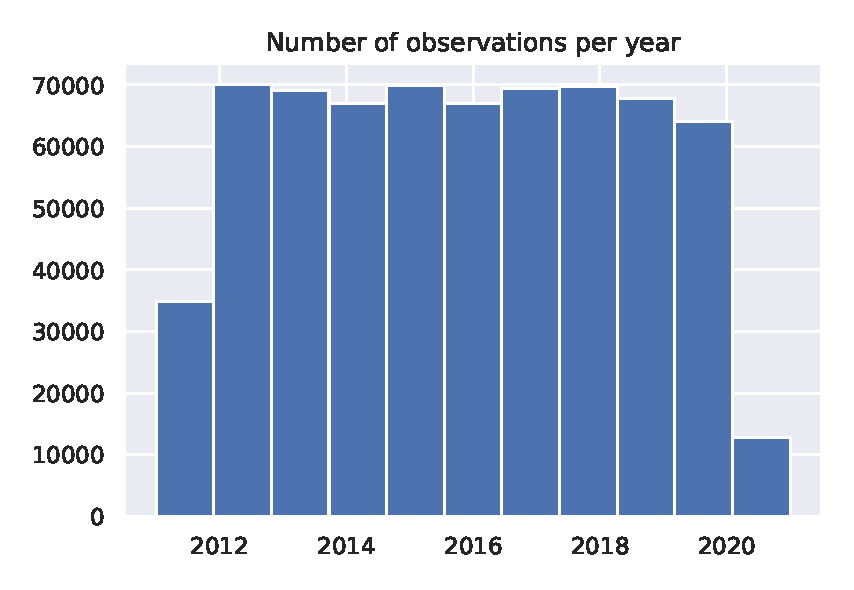
\includegraphics[width=0.47\textwidth]{histogram.eps}
    \end{center}
    \caption{Number of hourly measurements per year. In 2011, only half of the monitoring stations worked.}
    \label{fig:histogram-obs-years}
\end{figure}

\begin{enumerate}
    \item Analisar sazonalidade. Adicionar termo seno e cosseno de forma que
    exista sazonalidade diária, isto é, 
    $$
    \text{hour\_sin} = \sin(2\pi \text{ hour}/24)
    $$
    \item Create variable season.   
\end{enumerate}